Many insights described in previous chapters were obtained from experimentation and observation of pictures, videos, and interaction with the dynamic geometry of Poncelet configurations. Dozens of notebooks and 100s of small interactive apps were written with \cite{mathematica_v10}. Most of digital artifacts have been assembled in 
\cite{reznik2021-observable-media}.

To further facilitate exploratory discovery of invariants and locus properties of 3-periodic families, we developed a javascript-based locus visualization app \cite{darlan2020-app}.

A typical screenshot of the application is depicted in \cref{fig:09-screenshot}. The dark area is where the animated triangle family is rendered. To its left are ``channel controls'', divided up in four identical areas, which select features to be computed in real time. 

\begin{figure}
    \centering
    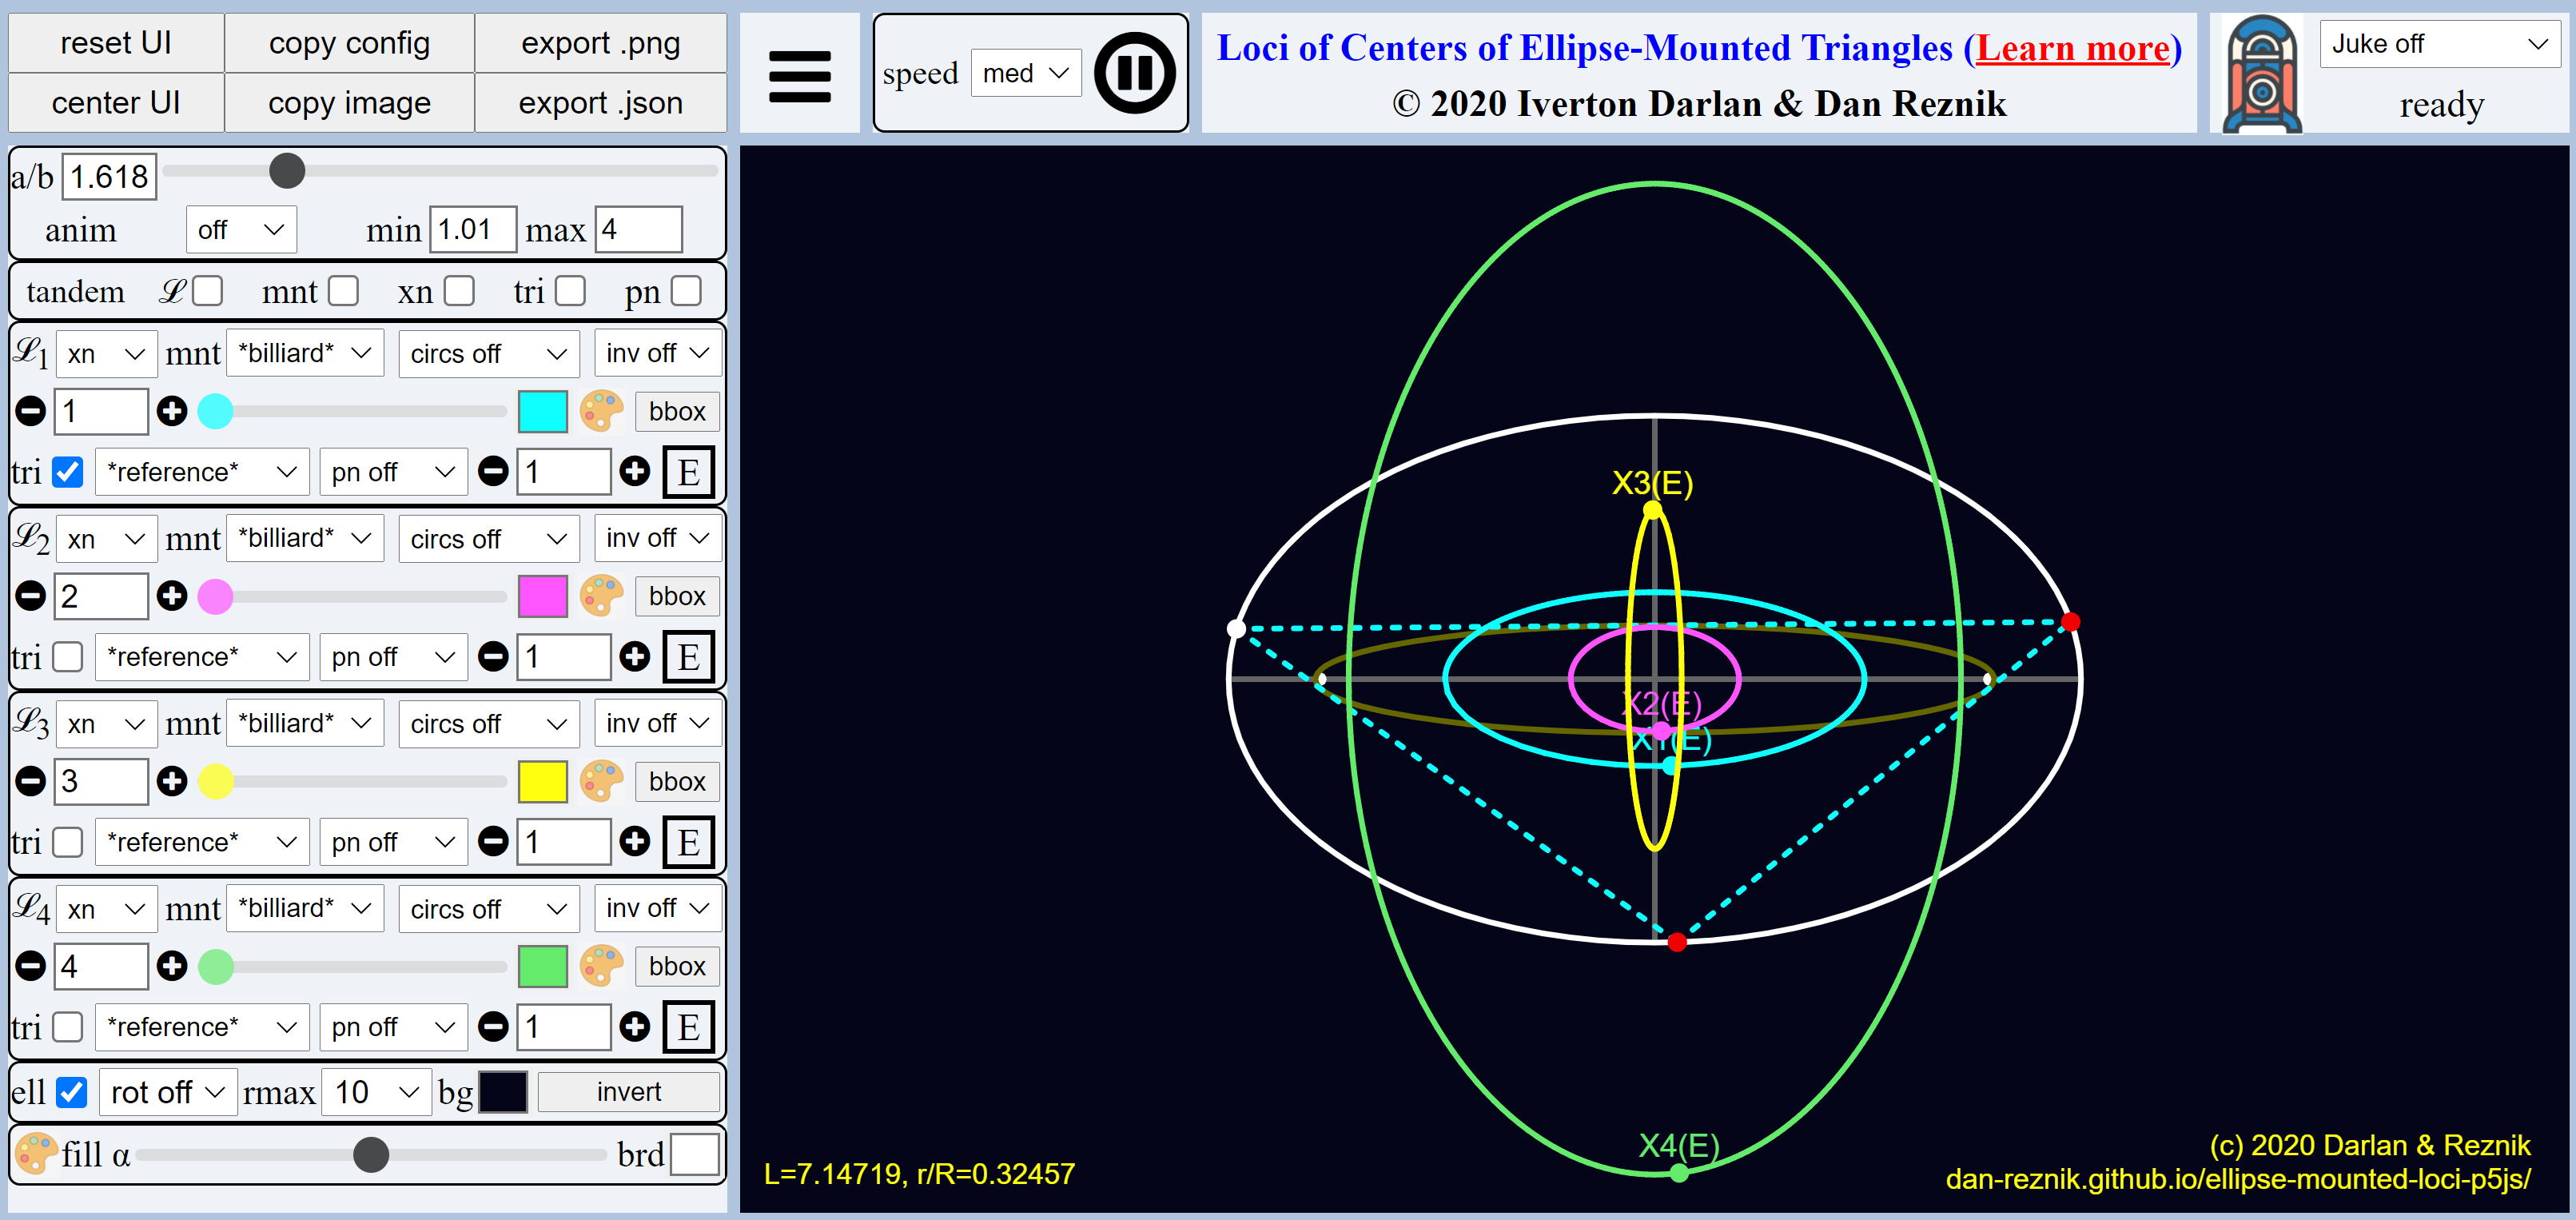
\includegraphics[width=\textwidth]{chap_09/pics/pics_09_010_screenshot.png}
    \caption{Locus Visualization app to explore 3-periodic families. Shown are the loci of $X_k$, $k=$1,2,3,4, over billiard 3-periodics. The ``(E)'' suffix indicated they are numerically ellipses. \href{https://bit.ly/3yV8caF}{Live}}
    \label{fig:09-screenshot}
\end{figure}

The most common usage pattern is depicted in \cref{fig:09-flow}, namely: the user selects (i) a triangle family (Poncelet or ellipse-mounted, see below); (ii) the triangle on which computations will be made (the default is ``reference'' but dozens of derived triangles can be chosen); (iii) the locus type, i.e., whether one wishes to trace out a triangle center, a vertex, an envelope, etc., and (iv) which triangle center should the locus be drawn for. The first one thousand triangle centers listed in \cite{etc} are currently supported.

\begin{figure}
    \centering
    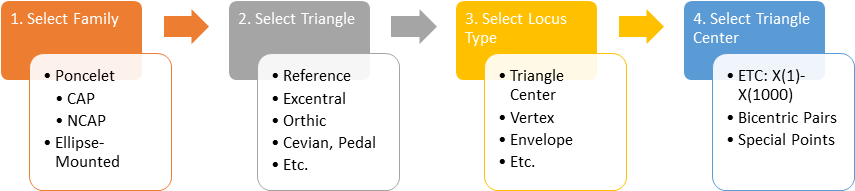
\includegraphics[width=\textwidth]{chap_09/pics/pics_09_020_workflow.png}
    \caption{Caption}
    \label{fig:09-flow}
\end{figure}

In the sections below we describe the main functions of the user interface.

